	\section{balance equation}
	\subsubsection{Ohm's Law}
		% Exercise Chapter 1, Aufgabe 2
		...bitte noch übertragen...
		\subsubsection{Heat conduction in 1D}
		% Exercise Chapter 1, Aufgabe 3
		\begin{itemize}
			
			\item Formulate the stationary het balance equation for a 1D system (slender rod). Genommen wird die Allgemeine Wärmeleitungsgleichung $\frac{\partial w}{\partial t}= -\nabla \cdot j_W+q_W$ und diese Vereinfacht, da Stationär und 1D ergibt es $0= -\frac{\partial j_W}{\partial x}+q_W$
			
			\item Formulate Fourier's law of heat conduction in 1D. Dies ist Allgemein $j_W=-\lambda \cdot \nabla T$ und im 1D $j_W=-\lambda \frac{\partial T}{\partial x} T$
			
			\item Solve this system of 2 ODEs of $1^{st}$ order for following conditions: a Al rod of length L=20cm , cross section $A=1cm^2$ and specific heat conductivity 
			$ \lambda = 240 W/(Km) $ 
			is cooled to $25^\circ C$ on its right hand side and heated on the lhs with a heat flux density of $ 36 kW/m^2 $ (candle).
			Es gilt das Fourier's law in die balance equation einzusetzen ergibt $ 0=\lambda \frac{\partial^2T}{\partial x^2}+q_W$, da es keine Quelle oder Senke hat gilt $q_W=0$. Löst man diese Differentialgleichung ergibt es $T(x)=C_1x+C_2$. An der Stelle (x=0) gilt das Fourier's law, also gilt $j_W=-\lambda \frac{\partial T}{\partial x} = 36000 = -240 \frac{\partial T}{\partial x } \Rightarrow \frac{\partial T}{\partial x}=-150 \frac{K}{m} =C_1$ und auch gegeben ist $25^\circ C$ an der Stelle x=0.2m. Damit $C_2$ ausrechnen ergibt  $ T(0.2)= -150 \frac{K}{m} \cdot 0.2m+C_2=25^{\circ} C $. Allgemein ergibt sich die Gleichung $ T(x)= -150 \frac{K}{m} \cdot x [m] + 25^{\circ} C $.
			
			\item Neu sind beide Seiten sind $25^\circ K$ Nun kommt zusätzlich noch eine Wärmequellerate für $500 kW/m^3$ nun gibt es $ -\lambda \frac{\partial^2T}{\partial x^2}=q_W$ löst man diese Partielle DGL ergibt es $T(x)=\frac{1}{2}\frac{-q_W}{\lambda} x^2+C_1x+C_2$ Setzt man die Randbedingungen ein ergibt es $T(x)=\frac{1}{2}\frac{q_W}{\lambda}(Lx-x^2)+T_0$
			
			
		\end{itemize}



	\subsubsection{Gauss Theorem}
	kubischer Würfel [1m, 1m, 1m] in 3d\\
	Vektorfeld: $v = v_0 (\frac{x_1}{a}, \frac{x_2}{a}, 0)^T$ mit $v_0 = 0.1 m/s$
	und $a = 1m$\\
	
	\textbf{sketch flow field in $x_1$, $x_2$-plane}\\
	
	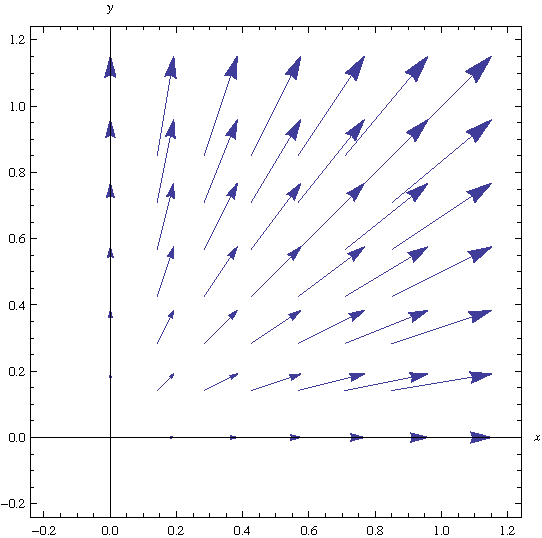
\includegraphics[scale=0.5]{images/gauss.pdf}\\ % weg mit dem figure plunder
	Vectorfield\\
	
	
	\textbf{Fluss über Fläche berechnen}\\
	Fluss über alle Flächen summieren:\\
	Fläche unten $x_1$,$x_3$ bei $x_2 = 0$:
	\begin{align}
		\oint_{S} \vec u \cdot
		\vec n\; \mathrm dA = \frac{v_0}{a} \oint_{S} \begin{pmatrix}
			x_1\\ x_2\\ 0
		\end{pmatrix} \cdot
		\begin{pmatrix}
			0\\ -1\\ 0
		\end{pmatrix} \mathrm dA = \frac{v_0}{a} \int_{0}^{1} \int_{0}^{1} x_2 \mathrm
		dx_1 \mathrm dx_3 = \frac{v_0}{a} \int_{0}^{1} \int_{0}^{1} 0 \mathrm dx_1
		\mathrm dx_3 = 0
	\end{align}
	Fläche oben $x_1$,$x_3$ bei $x_2 = 1$:
	\begin{align}
		\oint_{S}
		\vec n\; \mathrm dA = \frac{v_0}{a} \oint_{S} \begin{pmatrix}
			x_1\\ x_2\\ 0
		\end{pmatrix} \cdot
		\begin{pmatrix}
			0\\ -1\\ 0
		\end{pmatrix} \mathrm dA = \frac{v_0}{a} \int_{0}^{1} \int_{0}^{1} x_2 \mathrm
		dx_1 \mathrm dx_3 = \frac{v_0}{a} \int_{0}^{1} \int_{0}^{1} 1 \mathrm dx_1
		\mathrm dx_3 = \frac{v_0}{a}
	\end{align}
	Fläche hinten $x_1$,$x_2$ bei $x_3 = 1$:
	\begin{align}
		\oint_{S} \vec u \cdot
		\vec n\; \mathrm dA = \oint_{S} \frac{v_0}{a} \begin{pmatrix}
			x_1\\ x_2\\ 0
		\end{pmatrix} \cdot
		\begin{pmatrix}
			0\\ 0\\ 1
		\end{pmatrix} \mathrm dA = \int_{0}^{1} \int_{0}^{1} 0 \mathrm dx_1 \mathrm
		dx_2 = 0
	\end{align}
	Sinngemäss für alle Flächen Durchziehen:
	\begin{align}
		I_{tot} = \frac{v_0}{a} + \frac{v_0}{a} + 0 + 0 + 0 + 0 = 2 \frac{v_0}{a}
	\end{align}
	
	Mit Gauss theorem über Fläche (einfacher):
	\begin{align}
		\int_V \nabla \vec u \; \mathrm dV = \int_V \nabla \begin{pmatrix}
			x_1\\ x_2\\ 0
		\end{pmatrix} \; \mathrm dV = \int_{V}
		\frac{\partial x_1}{\partial x_1} + \frac{\partial x_2}{\partial x_2} +
		\frac{\partial 0}{\partial x_3} \; \mathrm dV =
		\frac{v_0}{a}
		\int_{0}^{1}
		\int_{0}^{1}
		\int_{0}^{1} 1 + 1 + 0 \; \mathrm dx_1 \mathrm dx_2 \mathrm dx_3 = 2
		\frac{v_0}{a}
	\end{align}

\subsubsection{Elastic Energy Density} % Probeprüfung Aufgabe 5

Der Tensor $ \epsilon^{eng}=(1,-1,1,2,0,0)^T $ aufteilen in $ \epsilon^{iso} $ und $ \epsilon^{shear} $. 
\\
Man übersetzt den Tensor von eng Notation in einen normalen Tensor. 
\\
$ \epsilon^{ing}
=
\begin{pmatrix} 
1 \\ 
-1 \\
1 \\ 
2 \\
0 \\ 
0 \\ 
\end{pmatrix}
\rightarrow 
\begin{pmatrix} 
1 & 0 & 0 \\
0 & -1 & 1 \\
0 & 0 & 1 \\
\end{pmatrix}
=
\epsilon $
\\
Nun gilt es den Tensor $ \epsilon $ aufzuteilen
\\
$ \epsilon^{iso}=\frac{tr(\epsilon)}{3}\cdot \textbf{I} = \frac{1}{3}\cdot
\underbrace{tr\begin{pmatrix} 
	1 & 0 & 0 \\
	0 & -1 & 1 \\
	0 & 0 & 1 \\
	\end{pmatrix}}_1
\cdot
\begin{pmatrix} 
1 & 0 & 0 \\
0 & 1 & 0 \\
0 & 0 & 1 \\
\end{pmatrix}
\rightarrow
\epsilon^{eng}_{iso}=
\frac{1}{3}\cdot
\begin{pmatrix} 
1 \\ 
1 \\
1 \\ 
0 \\
0 \\ 
0 \\ 
\end{pmatrix}
$
\\
$ \epsilon^{shear}=\epsilon-\epsilon^{iso}=
\begin{pmatrix} 
1 & 0 & 0 \\
0 & -1 & 1 \\
0 & 0 & 1 \\
\end{pmatrix}
-
\frac{1}{3}
\begin{pmatrix} 
1 & 0 & 0 \\
0 & 1 & 0 \\
0 & 0 & 1 \\
\end{pmatrix}
=
\frac{1}{3}
\begin{pmatrix} 
2 & 0 & 0 \\
0 & -4 & 1 \\
0 & 0 & 2 \\
\end{pmatrix}
=
\frac{1}{3}\cdot
\begin{pmatrix} 
2 \\ 
-4 \\
2 \\ 
6 \\
0 \\ 
0 \\ 
\end{pmatrix}
\rightarrow
\epsilon^{ing}_{shear}
\frac{1}{3}\cdot
\begin{pmatrix} 
2 \\ 
-4 \\
2 \\ 
6 \\
0 \\ 
0 \\ 
\end{pmatrix}
$

\subsubsection{2nd Rank Tensor Manipulation} % Exercises of Chapter 3

a) $\mathbf{C}=\mathbf{AB}$ $\Rightarrow$ $C_{ij}=A_{ik}B_{kj}$

Matrixmulitplikation weil die Dimension des resultierenden Tensors aus der
Anzahl Spalten des linken Tensors und der Anzahl Zeilen des Rechten Tensors
besteht. \qed

b) General heat conduction law $j_{th,k}=-\kappa_{kl}\frac{\partial
	T}{\partial x_l}$ Prove that the isotropic law is recovered by using the
specific 2nd Rank Tensor $\kappa_{kl}=\kappa \delta_{kl}$

$K_{kl}$ Einsetzen. In diesem Fall ist das Korneckerdelta eine $1$. Deshalb
ergibt sich $-\kappa \frac{\partial T}{\partial x_k}$ \qed

c) Show that the 2nd Rank Unit Tensor $\mathbf{I}$ has the same form in each
coordinate system.$\Rightarrow$ Orthogonal

Transformation eines Einheitstensors: $\mathbf{I}'=R\mathbf{I}R'\Rightarrow$.
$I_{il}'=R_{ij}\delta_{jk}R_{kl}^T = R_{ij}R_{jl}^T=\delta_{il}=I_{il}$ \qed



d) Prove tr $\mathbf{E}=\mathbf{E : I}$
Component $\Rightarrow$ $E_{ij}\delta_{ij}=E_{ii}$ \qed

e) Prove every 2nd Rank can be written as symmetric and asymmetric tensor.

$\mathbf{A}=\frac{1}{2}\left(\mathbf{A} + \mathbf{A}^T\right)+
\frac{1}{2}\left(\mathbf{A}-\mathbf{A}^T\right) = \mathbf{A}$ \\
$\mathbf{A}=\left(\mathbf{A}_1^{sym}-\mathbf{A}_1^{sym}\right)=\left(\mathbf{A}_2^{sym}-\mathbf{A}_2^{sym}\right)$
\\
$0=\left(\mathbf{A}_1^{sym}-\mathbf{A}_2^{sym}\right)+\left(\mathbf{A}_1^{asym}-\mathbf{A}_2^{asym}\right)$
\\
$0=\mathbf{C}^{sym}+\mathbf{C}^{asym}$ $\Rightarrow$
$\mathbf{A}_1^{sym}=\mathbf{A}_2^{sym}$ $\Rightarrow$
$\mathbf{A}_1^{asym}=\mathbf{A}_2^{asym}$ \qed


f) \colorbox{red}{Kucksch du selber!, nicht realistisch!}




\subsection{Exercises of Chapter 3c)}

\subsubsection{4th Rank Tensor Manipulation}


$I_{ijkl}A_{kl}=\frac{1}{2}(\delta_{ik}\delta_{kl}+\delta_{il}\delta_{jk})A_{kl}=\frac{1}{2}(A_{ij}+A_{ji})=A_{ij}$
\\
\\
$ \mathbb{I} $ und $ \mathbb{E} $ sind unabhänig vom Koordinatensystem wenn diese isotrop sind

$ I'_{mnpq}=R_{mi}R_{nj}R_{pk}R_{ql}I_{ijkl} = \frac{1}{2}(R_{mi}\delta_{ik}R_{pk}R_{nj}\delta_{jl}R_{ql} + R_{mi}\delta_{il}R_{ql}R_{nj}\delta_{jk}R_{pk})= \frac{1}{2}(R_{mi}R^T_{ip}R_{nj}R^T_{jq}+R_{mi}R^T_{iq}R_{nj}R^T_{jp})= \frac{1}{2}(\delta_{mp}\delta_{mq}\delta_{np})=I_{mnpq} $ dasselbe gilt auch für $ E'_{mnpq}=E_{mnpq}$


\subsubsection{2D Carbon Plate Thermal Conduction} % Exercise Week 6

a) Conductivity Tensor of the problem

\begin{align}
k_{ij}=\begin{pmatrix}
50 & 0 & 0 \\
0 & 250 & 0 \\
0 & 0 & 250 
\end{pmatrix}
\end{align}
\qed
\begin{align}
a = \frac{1}{\sqrt{\sigma_1}} = \frac{1}{\sqrt{50}} \text{ und } b =
\frac{1}{\sqrt{\sigma_2}} = \frac{1}{\sqrt{250}}
\end{align}

\begin{center}
	Ellipse Conductivity Tensor Quadrik:\\
	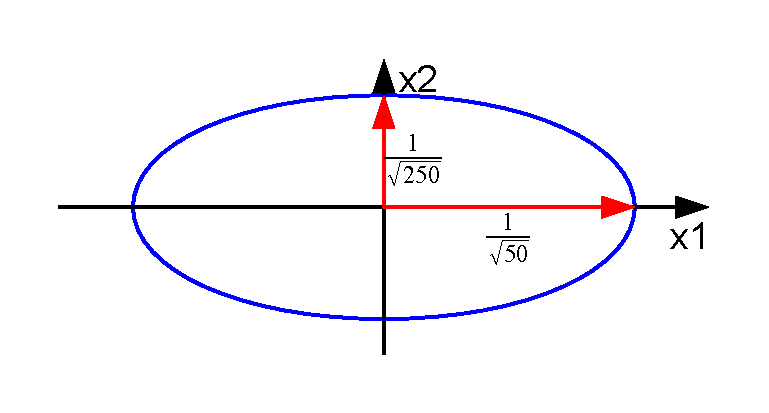
\includegraphics[scale=0.8]{images/quadrik_2d_ellipse_uebung.pdf}\\
	Kommentar zu Grafik: x2,x3 und senkrechte Striche einfügen\\
\end{center}
Bemerkungen: blauer Kreis zeigt den Widerstand, ist dieser Gross leitet es schlecht, ist der Widerstand klein leitet es gut.
\\
\\
b) Transformation $30^\circ$
\begin{align}
k_{ij}'=RkR^{T}
\end{align}

\begin{align}
\phi=+30^\circ
\end{align}

\begin{align}
k_{ij}'=\begin{pmatrix}
\cos{\phi} & -\sin{\phi} & 0 \\
\sin{\phi} & \cos{\phi} & 0 \\
0 & 0 & 1
\end{pmatrix}
\cdot
\begin{pmatrix}
50 & 0 & 0 \\
0 & 250 & 0 \\
0 & 0 & 250 
\end{pmatrix}
\cdot
\begin{pmatrix}
\cos{\phi} & \sin{\phi} & 0 \\
-\sin{\phi} & \cos{\phi} & 0 \\
0 & 0 & 1
\end{pmatrix}
\end{align}

\begin{align}
k_{ij}'=\begin{pmatrix}
100 & -86.60 & 0 \\
-86.60 & 200 & 0 \\
0 & 0 & 250
\end{pmatrix}
\end{align}
\qed

c) Heatflow in x1 Direction, $30^\circ$ Rotated Material

Alle Ableitungen bis auf $\frac{\partial T}{\partial x1}=a$ sind 0


\begin{align}
j_i=-k_{ij} \frac{\partial T}{\partial x_j}
\end{align}

\begin{align}
\vec{j}=\begin{pmatrix}
100 \\
-86.6 \\
0
\end{pmatrix}
\cdot -a
\end{align}

\qed
d) Ellipsoid

\begin{center}
	Gedrehter Tensor (nicht im Hauptachsensystem):\\
	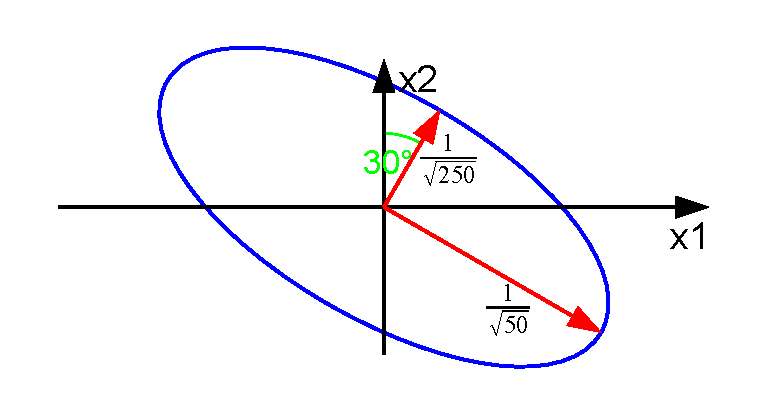
\includegraphics[scale=0.8]{images/quadrik_2d_ellipse_uebung_rotation.pdf}\\
	Kommentar zur Grafik: x2,x3 und schräge Striche einfügen\\
\end{center}

e) Determine the resistivity $r_{12}$

\begin{align}
r_{ij}=\frac{1}{k_{ij}}=\begin{pmatrix}
\frac{1}{k_{11}} & 0 & 0 \\
0 & \frac{1}{k_{22}} & 0 \\
0 & 0 & \frac{1}{k_{33}}
\end{pmatrix}
\end{align}

\begin{align}
r_{ij}'=Rr_{ij}R^{T} = \begin{pmatrix}
16 & 6.9 & 0 \\
6.9 & 8 & 0 \\
0 & 0 & 4
\end{pmatrix}
10^{-3}[\frac{mK}{W}] 
\end{align}
\qed




\subsubsection{Eletrical Tin}
Write down the conductivity Tensor:\\
(Bemerkung: andere Materialwerte sind im Skript, Kapitel 4 auf der Seite 6 zu finden)

\begin{align}
\sigma_{ij} = \frac{1}{\rho_{ij}}= \begin{pmatrix}
101 & 0 & 0 \\
0 & 101 & 0 \\
0 & 0 & 69.9 
\end{pmatrix}
10^5 [\frac{S}{m}]
\end{align}



a) Calculate the magnitude and the direction of the current density

\begin{align}
j_i=\sigma_{ij}E_j
\end{align}

Multiplizieren mit Feld...
\\... z.B. $ j_i=\sigma_{ij}E_j = \sigma_{ij} = \frac{1}{\rho_{ij}}= \begin{pmatrix}
101 & 0 & 0 \\
0 & 101 & 0 \\
0 & 0 & 69.9 
\end{pmatrix} 10^5 [\frac{S}{m}] 
\begin{pmatrix}
0 \\
0.5 \\
0.866 \\
\end{pmatrix} [\frac{V}{m}] = 
\begin{pmatrix}
0 \\
5.05 \\
6.05 \\
\end{pmatrix} 10^5 [\frac{A}{m^2}]$



Danach Vektorbetrag und Winkel berechnen. :-)\\

Vektorbetrag: 

\begin{align}
j_i=\sqrt{j_x^2+j_y^2+j_z^2}
\end{align}
... z.B. $\sqrt{ 0^2+(5.05 \cdot 10^5)^2+(5.05 \cdot 10^5)^2 } = 7.88 [\frac{A}{mm^2}]$ 
\\
\\
Winkel:

\begin{align}
\tan{\alpha}=\frac{Gegenkathete}{Ankathete} \Rightarrow \alpha=arctan(\frac{Gegenkathete}{Ankathete})
\end{align}
... z.B. $ \alpha=arctan(\frac{Gegenkathete}{Ankathete}) = arctan(\frac{6.05 \cdot 10^5}{5.05 \cdot 10^5}) = 50^\circ $


c) Ellipsoid zeichnen



\qed


\subsection{Exercise}
\subsubsection{Useful formulas}

Gradient von $ (\frac{1}{r}) $  with $ r=\sqrt{x^2+y^2+z^2} $

Anwenden von der Produktregel eines Gradient, siehe Formel \ref{eqn:ProduktregelEinesGradientMitPotenzen} auf Seite \pageref{eqn:ProduktregelEinesGradientMitPotenzen}

$ \nabla(\frac{1}{r}) = -\frac{\vec{r}}{r^3}$
\\
$ \nabla(\frac{1}{r^2}) = -2\frac{\vec{r}}{r^4}$
\\
$ \nabla(\frac{1}{r^3}) = -3\frac{\vec{r}}{r^5}$

\subsubsection{The electrical field}

Info A\\
Berechnung von curl von einer Punktladung.\\ 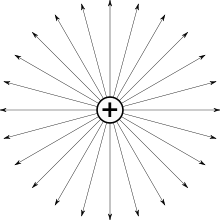
\includegraphics[scale=0.2]{images/punktladung.png}
\label{fig:Punktladung}

$ \vec{E}(\vec{r})=\frac{q}{4\Pi\epsilon_0}\frac{\vec{r}}{r^3}\sim \frac{\vec{r}}{r^3} $
\\
$ \vec{\nabla}\times\vec{E}\approx\vec{\nabla}\times(\frac{\vec{r}}{\vec{r^3}})=\frac{\vec{1}}{r^3}(\vec{\nabla}\times\vec{r})+\vec{r}\times(\vec{\nabla}(\frac{1}{r^3}))=-\frac{3}{r^5}(\vec{r}\times\vec{r})=0 $

Info B\\
$ k=\frac{1}{4\pi\epsilon_0} $

Info C\\


Info D\\

\subsubsection{Polar Molecules (Torque and force)}

torque on molecule by an electrical field\\

$ \vec{F}=q\cdot\vec{E}$\\

$ \vec{M}=\vec{r}\cdot\vec{F}$\\

$ \vec{M}=\vec{p}\times\vec{E}$\\

Non uniform E-Field\\

\begin{align}
\vec F = \begin{pmatrix}
P_x \frac{\partial E_x}{\partial x} + P_y \frac{\partial E_x}{\partial y} + P_z
\frac{\partial E_x}{\partial z}\\
P_x \frac{\partial E_y}{\partial x} + P_y \frac{\partial E_y}{\partial y} + P_z
\frac{\partial E_y}{\partial z}\\
P_x \frac{\partial E_z}{\partial x} + P_y \frac{\partial E_z}{\partial y} + P_z
\frac{\partial E_z}{\partial z}\\
\end{pmatrix}
= \operatorname{grad} (\vec E) \cdot \vec p
\end{align}


\subsection{Elasticity}
\begin{minipage}{3cm}
	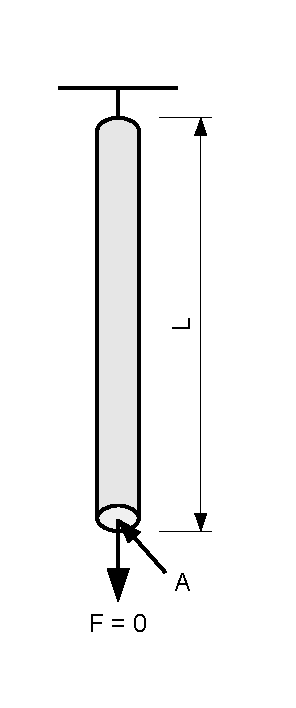
\includegraphics[scale=0.6]{images/elasticity_robe.pdf}
\end{minipage}
\hfill
\begin{minipage}{14cm}
	Balance equation: $0 = \frac{\partial \sigma_{11}}{\partial x} + \rho g_1$\\
	Material law: $\epsilon_{11} = \frac{\partial u(x)}{\partial x}$ with
	$\sigma_{11} = E \cdot \epsilon_{11}$\\
	Boundary conditions: $\sigma_{11} (L) = \frac{F}{A}$, $u(0)= 0$\\
	
	DGL aufstellen: $\frac{\partial \sigma (x)}{\partial x} = - \rho g$ $\mid$ $\int
	dx$\\
	DGL lösen: $\sigma (x) = - \rho g x + \sigma_0$\\
	Boundary Conditions bei L: $\sigma (L) = \frac{F}{A} = \frac{0}{A} = 0$\\
	BC in DGL einsetzen: $\sigma (L) = - \rho g L + \sigma_0 = 0$\\
	Auflösen: $\sigma_0 = \rho g L$\\
	In DGL einsetzen: $\sigma (x) = - \rho g x + \rho g L = \rho g (L-x)$\\
	Material law: $\epsilon (x) = \frac{\rho g}{E} (L-x)$\\
	Aus Material law: $\frac{\partial u(x)}{\partial x} = \epsilon (x) = \frac{\rho
		g}{E} (L-x)$ $\mid$ $\int dx$\\
	Deformation: $u(x) - u(0) = \int\limits_{0}^{x} dx' \cdot \epsilon(x') =
	\int\limits_{0}^{x} \frac{\rho g}{E} (L-x) dx = \frac{\rho g}{E} (x \cdot L -
	\frac{1}{2} \cdot x^2) = \frac{\rho g}{E} \cdot x(L-\frac{x}{2})$, wobei $u(0) =
	0$\\
	Wichtig x' statt x verwenden, u(x) ist gemeint dasss wir die Dehnung von 0 bis
	zu einem Punkt zwischen 0 und L integrieren!\\
	
\end{minipage}
\textbf{Maximaler Stress} tritt an der Aufhängung an Punkt $x = 0$ auf:\\
$\sigma(0) = - \rho g (L-x) = \rho g L = \frac{m \cdot g}{A}$\\
Einheitenkontrolle: $[\rho \cdot g \cdot L] = \frac{kg}{m^3} \cdot
\frac{m}{s^2} \cdot m = \frac{kg}{m \cdot s^2}$\\
$[m \cdot g \cdot \frac{1}{A}] = kg \cdot \frac{m}{s^2} \cdot \frac{1}{m^2} =
\frac{kg}{m \cdot s^2}$\\
\subsubsection{Nochmals das gleiche mit Gewicht}
$F \neq 0$ $\to$ $\sigma(L) = \frac{M
	g}{A}$\\
DGL aufstellen: $\frac{\partial \sigma (x)}{\partial x} = - \rho g$ $\mid$
$\int dx$\\
DGL lösen: $\sigma (x) = - \rho g x + \sigma_0$\\
Boundary Conditions bei L: $\sigma (L) = \frac{F}{A} = \frac{M g}{A}$\\
BC in DGL einsetzen: $\sigma (L) = - \rho g L + \sigma_0 = \frac{M g}{A}$\\
Auflösen: $\sigma_0 = \rho g L + \frac{M
	g}{A}$\\
In DGL einsetzen: $\sigma (x) = - \rho g x + \rho g L + \frac{M g}{A}= \rho g
(L-x) + \frac{M g}{A}$\\
Material law: $\epsilon (x) = \frac{\rho g}{E} (L-x) + \frac{M g}{E A}$\\
Aus Material law: $\frac{\partial u(x)}{\partial x} = \epsilon (x) = \frac{\rho
	g}{E} (L-x) + \frac{M g}{E A} =  \frac{g}{E} (\rho L + \frac{M}{A} - \rho x) $
$\mid$ $\int dx$\\
Deformation: $u(x) - u(0) = \int\limits_{0}^{x} \epsilon(x) dx =
\int\limits_{0}^{x} \frac{g}{E} (\rho L + \frac{M}{A} - \rho x) dx =
\frac{g}{E} \cdot x \left( \left( L \rho + \frac{M}{A} \right) -
\frac{x \rho}{2}\right)$, wobei $u(0) = 0$\\

\subsubsection{Spring Constant (Federkonstante)}
Definition Federkonstante: $F = d \cdot \Delta u $\\
$\sigma = \frac{F}{A}$ $\Rightarrow$ (siehe Übung oben) $u(x) = \frac{F}{A E}
x$\\
Für 1D und isotrop über ganzes Gummiband: $x = L$\\
$\Delta u = \frac{F L}{A E}$\\
Aus $F = d \cdot \Delta u $ ergibt sich: $d = \frac{A E}{L}$

\subsection{Beispiel Teil 2 (Strain, Stress, \ldots)} % Exercises Week 9

\subsubsection{Pure Shear Stress}

\textbf{Momentum flux}\\
\begin{minipage}{6cm}
	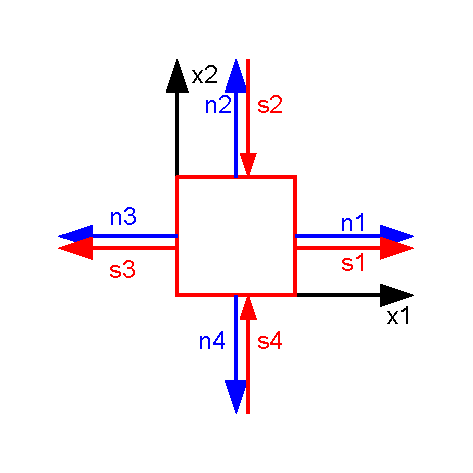
\includegraphics[scale=0.8]{images/pure_shear_stress_1.pdf}
\end{minipage}
\hfill
\begin{minipage}{14cm}
	Gegeben: $\sigma = \begin{pmatrix}
	s & 0 & 0\\
	0 & -s & 0\\
	0 & 0 & 0\\
	\end{pmatrix} $\\
	cutting forces on each face:\\
	$s_1 = \sigma \vec n_1 = \begin{pmatrix}
	s & 0\\
	0 & -s\\
	\end{pmatrix} \begin{pmatrix}
	1\\
	0\\
	\end{pmatrix} = \begin{pmatrix}
	s\\
	0\\
	\end{pmatrix}$\\
	
	$s_2 = \sigma \vec n_2 = \begin{pmatrix}
	s & 0\\
	0 & -s\\
	\end{pmatrix} \begin{pmatrix}
	0\\
	1\\
	\end{pmatrix} = \begin{pmatrix}
	0\\
	-s\\
	\end{pmatrix}$\\
	
	$s_3 = \sigma \vec n_3 = \begin{pmatrix}
	s & 0\\
	0 & -s\\
	\end{pmatrix} \begin{pmatrix}
	-1\\
	0\\
	\end{pmatrix} = \begin{pmatrix}
	-s\\
	0\\
	\end{pmatrix}$\\
	
	$s_4 = \sigma \vec n_4 = \begin{pmatrix}
	s & 0\\
	0 & -s\\
	\end{pmatrix} \begin{pmatrix}
	0\\
	-1\\
	\end{pmatrix} = \begin{pmatrix}
	0\\
	s\\
	\end{pmatrix}$
	
\end{minipage}

\textbf{Transform}\\
Transformation as usual:
\begin{align}
	\sigma'_{kl}=R_{ki}R_{lj}\sigma_{ij}=R_{ki}\sigma_{ij}R_{jl}^T \\
	R_{kl}=\begin{pmatrix} 
		\cos \alpha & -\sin \alpha & 0 \\
		\sin \alpha &  \cos \alpha & 0 \\            
		0        &  0           & 1
	\end{pmatrix}
\end{align}

Resultat:

\begin{align}
	\sigma'_{kl}=\begin{pmatrix}
		0 & s & 0 \\
		s & 0 & 0 \\
		0 & 0 & 0
	\end{pmatrix}
\end{align}

\begin{minipage}{6cm}
	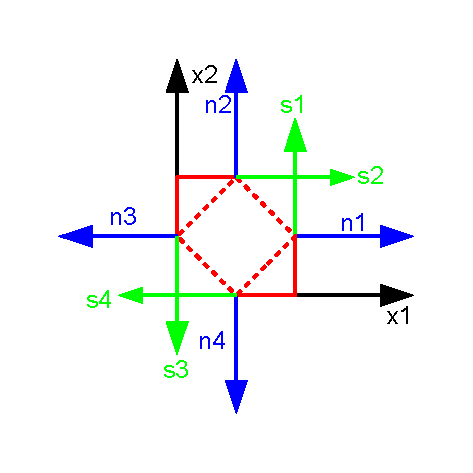
\includegraphics[scale=0.8]{images/pure_shear_stress_2.pdf}
\end{minipage}
\hfill
\begin{minipage}{14cm}
	cutting forces on each face:\\
	$s_1 = \sigma \vec n_1 = \begin{pmatrix}
	0 & s\\
	s & 0\\
	\end{pmatrix} \begin{pmatrix}
	1\\
	0\\
	\end{pmatrix} = \begin{pmatrix}
	0\\
	s\\
	\end{pmatrix}$\\
	
	$s_2 = \sigma \vec n_2 = \begin{pmatrix}
	0 & s\\
	s & 0\\
	\end{pmatrix} \begin{pmatrix}
	0\\
	1\\
	\end{pmatrix} = \begin{pmatrix}
	s\\
	0\\
	\end{pmatrix}$\\
	
	$s_3 = \sigma \vec n_3 = \begin{pmatrix}
	0 & s\\
	s & 0\\
	\end{pmatrix} \begin{pmatrix}
	-1\\
	0\\
	\end{pmatrix} = \begin{pmatrix}
	0\\
	-s\\
	\end{pmatrix}$\\
	
	$s_4 = \sigma \vec n_4 = \begin{pmatrix}
	0 & s\\
	s & 0\\
	\end{pmatrix} \begin{pmatrix}
	0\\
	-1\\
	\end{pmatrix} = \begin{pmatrix}
	-s\\
	0\\
	\end{pmatrix}$\\
	
\end{minipage}

\textbf{Trace}\\

\begin{align}
	\operatorname{tr}\sigma_{kl}=0 \\
	\operatorname{tr}\sigma'_{kl}=0 
\end{align}

$\Rightarrow$ Pure Shear Stress
\qed
\subsubsection{Stress in the Principal Axis System}
Gegeben:
\begin{align}
	\sigma=\begin{pmatrix}
		-\frac{2}{25} & 0 & \frac{36}{25} \\
		0 & 3 & 0 \\
		\frac{36}{25}& 0 & -\frac{23}{25}
	\end{pmatrix}
\end{align}

Find Eigenvalues:

\begin{align}
	\operatorname{eig}(\sigma)=\left(1,-2, 3\right) \operatorname{or}
	\left(1,3,-2\right)
\end{align}
Eigenwerte werden standardmässig nach Grösse geordnet (Reihenfolge jedoch nicht
relevant, ergibt anderes Koordinatensystem).


Resultat:

\begin{align}
	\sigma'=\begin{pmatrix}
		1 & 0 & 0 \\
		0 & 3 & 0 \\
		0 & 0 & -2
	\end{pmatrix}
\end{align}

Aufteilung des Stresstensor siehe Kapitel \ref{stressdecomposition} auf Seite
\pageref{stressdecomposition}!

\subsubsection{Deformation Strain State}\label{9.3} % Exercises Week 9.3
Gegeben Deformation: $u = (a \cdot x_2, b \cdot x_2, 0)^T$

b) Gradient der Deformation: $e_ij= \frac{\partial u_i}{\partial x_j} => e =
\begin{bmatrix}
0 & a & 0\\
0 & b & 0\\
0 & 0 & 0\\
\end{bmatrix}$\\
In symmetrischen und antisymmetrischen Teil splitten: $e = e^{sym} + e^{anti}=
\begin{pmatrix}
0 & a/2 & 0\\
a/2 & b & 0\\
0 & 0 & 0\\
\end{pmatrix}
+
\begin{pmatrix}
0 & a/2 & 0\\
-a/2 & 0 & 0\\
0 & 0 & 0\\
\end{pmatrix}$\\
Symmetrischer Part: $\epsilon = \begin{pmatrix}
0 & a/2 & 0\\
a/2 & b & 0\\
0 & 0 & 0\\
\end{pmatrix}$, da $\epsilon_{33} = \epsilon_{13} = \epsilon_{23}= 0$ $\rightarrow$ plane
strain\\
Antisymmetrischer Part: $\gamma = \begin{pmatrix}
0 & a/2 & 0\\
-a/2 & 0 & 0\\
0 & 0 & 0\\
\end{pmatrix}$ $\rightarrow$ Korrespondiert zu einer Drehung um die z-Achse mit
dem Winkel $\Phi \approx -\frac{a}{2}$ (für kleine Winkel), Drehmatrix:
$R_z(\alpha) = \begin{pmatrix} \cos \alpha & -\sin \alpha & 0 \\
\sin \alpha &  \cos \alpha & 0 \\            
0        &  0           & 1
\end{pmatrix}$

c) Find a deformation vector $u(x)$ reproducing the symmetric part of the strain
tensor that is as symmetric as possible with respectq to $x_1$ and $x_2$. Depict
this new deformation graphically and interpret the relation of the old
deformation, the antisymmetric part in the light of the new deformation.\\

$u(x) = \epsilon \cdot \begin{pmatrix} x_1\\ x_2\\ x_3\\ \end{pmatrix} =
\begin{pmatrix} 0 & a/2 & 0\\
a/2 & b & 0\\
0 & 0 & 0\\
\end{pmatrix} \cdot \begin{pmatrix} x_1\\ x_2\\ x_3\\ \end{pmatrix} =
\begin{pmatrix}
\frac{a}{2} \cdot x_2\\ \frac{a}{2} \cdot x_1 + b \cdot x_2\\ 0\\ \end{pmatrix}$

d) Tensor aufteilen (Volumenerhaltung (volume preserving))\\
$\epsilon =
\underbrace{
	\begin{pmatrix}
	b/3 & 0 & 0\\
	0 & b/3 & 0\\
	0 & 0 & b/3\\
	\end{pmatrix}
}_{\text{Volumenänderung}} +
\underbrace {
	\begin{pmatrix}
	-b/3 & a/2 & 0\\
	a/2 & 2b/3 & 0\\
	0 & 0 & -b/3\\
	\end{pmatrix}}_{\begin{matrix} Spur = 0\\ \text{keine Volumenänderung}\\
	\end{matrix}}$

e) Relative Volumenänderung: $\frac{\Delta V}{V} = \frac{b}{3} + \frac{b}{3} +
\frac{b}{3} = b$

\subsection{Beispiel Elastizität II} % Exercises of Chapter 10

\subsubsection{Elasticity Tensor and Projections} % Aufgabe 10.1
Show that:
\begin{align}\label{eq:10.1a}
	\frac{1}{3} \mathbb{E} : \frac{1}{3} \mathbb{E} = \frac{1}{3}
	\mathbb{E}
\end{align}
Definition E: $E_{ijkl} = \delta_{ij} \delta_{kl}$\\
Formel \ref{eq:10.1a} in Komponenten repräsentation:
\begin{align}
	\frac{1}{9} E_{ijkl} E_{klpq} = \frac{1}{9} \delta_{ij} \delta_{kl} \delta_{kl}
	\delta_{pq} = \frac{1}{9} \delta_{ij} \delta_{kk} \delta_{pq} = \frac{1}{3}
	E_{ijpq}
\end{align}

\subsubsection{E-Modul Along Special Directions} % Aufgabe 10.4

\textbf{E-Modul Silicon along one axis}\\
Determine the E-module for Si in the direction along one of the cubic
axes\\

Spannung in [1, 0, 0] Richtung: $\sigma = (\sigma_{11}, 0, 0, 0, 0, 0)^T$\\

Beziehung gegeben: $\sigma = \mathbb{C} \epsilon$ Umgeformt: $\epsilon =
\mathbb{C}^{-1} \sigma$\\

Für $\mathbb{C}$ gilt (fliegt von SkriptHimmel):
\begin{align}
	\mathbb{C}^{cube} = \begin{pmatrix}
		C_{11} & C_{12} & C_{12} & 0 & 0 & 0\\
		C_{12} & C_{11} & C_{12} & 0 & 0 & 0\\
		C_{12} & C_{12} & C_{11} & 0 & 0 & 0\\
		0 & 0 & 0 & C_{44} & 0 & 0\\
		0 & 0 & 0 & 0 & C_{44} & 0\\
		0 & 0 & 0 & 0 & 0 & C_{44}\\
	\end{pmatrix}
\end{align}
with:
\begin{align}
	\begin{pmatrix}
		C_{11} = 166 GPa\\
		C_{12} = 64 GPa\\
		C_{44} = 79.6 GPa\\
	\end{pmatrix}
\end{align}
Dabei interessiert uns nur der obere Teil:
\begin{align}
	\mathbb{C} = \begin{pmatrix}
		C_{11} & C_{12} & C_{12}\\
		C_{12} & C_{11} & C_{12}\\
		C_{12} & C_{12} & C_{11}
	\end{pmatrix}
\end{align}
Diesen Invertieren:
\begin{align}
	\mathbb{C}^{-1} = \begin{pmatrix}
		\frac{C_{11} + C_{12}}{C_{11}^2 + C_{11} \cdot C_{12} - 2 \cdot C_{12}^2} &
		\frac{-C_{11}}{C_{11}^2 + C_{11} \cdot C_{12} - 2 \cdot C_{12}^2} &
		\frac{-C_{11}}{C_{11}^2 + C_{11} \cdot C_{12} - 2 \cdot C_{12}^2}\\
		\frac{-C_{11}}{C_{11}^2 + C_{11} \cdot C_{12} - 2 \cdot C_{12}^2} &
		\frac{C_{11} + C_{12}}{C_{11}^2 + C_{11} \cdot C_{12} - 2 \cdot C_{12}^2} & 
		\frac{-C_{11}}{C_{11}^2 + C_{11} \cdot C_{12} - 2 \cdot C_{12}^2}\\
		\frac{-C_{11}}{C_{11}^2 + C_{11} \cdot C_{12} - 2 \cdot C_{12}^2} &
		\frac{-C_{11}}{C_{11}^2 + C_{11} \cdot C_{12} - 2 \cdot C_{12}^2} &
		\frac{C_{11} + C_{12}}{C_{11}^2 + C_{11} \cdot C_{12} - 2 \cdot C_{12}^2}
	\end{pmatrix}
\end{align}
Da alles ausser $\sigma_{11}$ gleich 0 ist, gilt:
\begin{align}
	\epsilon_{11} = C_{11} \sigma_{11}
\end{align}
Umgeformt und eingesetzt:
\begin{align}
	E_{[100]} = \frac{\sigma_{11}}{\epsilon_{11}} = \frac{1}{C_{11}} =
	\frac{C_{11}^2 + C_{11} \cdot C_{12} - 2 \cdot C_{12}^2}{C_{11} + C_{12}} = 130
	GPa
\end{align}


\textbf{E-Modul Silicon diagonal face}\\


Spannung in [1, 0, 0] Richtung: $\sigma = (\sigma_{11}, 0, 0, 0, 0, 0)^T$\\

Beziehung gegeben: $\sigma = \mathbb{C} \epsilon$ Umgeformt: $\epsilon =
\mathbb{C}^{-1} \sigma$\\


Stelle $\mathbb{C}$ mit

\begin{align}
	\mathbb{C}^{cube} = \begin{pmatrix}
		C_{11} & C_{12} & C_{12} & 0 & 0 & 0\\
		C_{12} & C_{11} & C_{12} & 0 & 0 & 0\\
		C_{12} & C_{12} & C_{11} & 0 & 0 & 0\\
		0 & 0 & 0 & C_{44} & 0 & 0\\
		0 & 0 & 0 & 0 & C_{44} & 0\\
		0 & 0 & 0 & 0 & 0 & C_{44}\\
	\end{pmatrix}
\end{align}

mit

\begin{align}
	\begin{pmatrix}
		C_{11} = 166 GPa\\
		C_{12} = 64 GPa\\
		C_{44} = 79.6 GPa\\
	\end{pmatrix}
\end{align}

Wechsle $\sigma$ in die Matrixnotation und drehe $\sigma$ um $\frac{\pi}{4}$
$[1,1,0]$

\begin{align}
	\sigma'=R \sigma R^{T}
\end{align}

Wechsle $\sigma$ wieder in Voigt-Notation

\begin{align}
	\sigma'=\begin{pmatrix}
		\frac{\sigma_{11}}{2} \\
		\frac{\sigma_{11}}{2} \\
		0 \\
		0 \\
		0 \\
		\sigma_{11}
	\end{pmatrix}
\end{align}

Wende $\mathbb{C}^{-1} \cdot \sigma'$ an um $\epsilon'$ zu erhalten

\begin{align}
	\epsilon'=\begin{pmatrix}
		0.00276 \cdot \sigma_{11} \\
		0.00276 \cdot \sigma_{11} \\
		-0.00213 \cdot \sigma_{11} \\
		0 \\
		0 \\
		0.01256 \cdot \sigma_{11}
	\end{pmatrix}
\end{align}

Wechsle $\epsilon'$ wieder in Matrix Notation und transformiere es auf um
$\frac{\pi}{4}$ zurück und wechsle wieder in Voigt Notation.

\begin{align}
	\epsilon=R^{T}\epsilon'R \\
	\epsilon=\begin{pmatrix}
		0.0059 \cdot \sigma_{11} \\
		-0.00038 \cdot \sigma_{11} \\
		-0.00213 \cdot \sigma_{11} \\
		0 \\
		0 \\
		0
	\end{pmatrix}
\end{align}

Rechne $E=\frac{\sigma_{11}}{\epsilon_{11}}$

\begin{align}
	E=\frac{\sigma_{11}}{0.0059 \cdot \sigma_{11}} \\
	E=169GPa
\end{align}

\subsection{Beispiel Structural Mechanics} % Übungsprüfung Problem 4

\begin{figure}[h]
	\begin{center}
		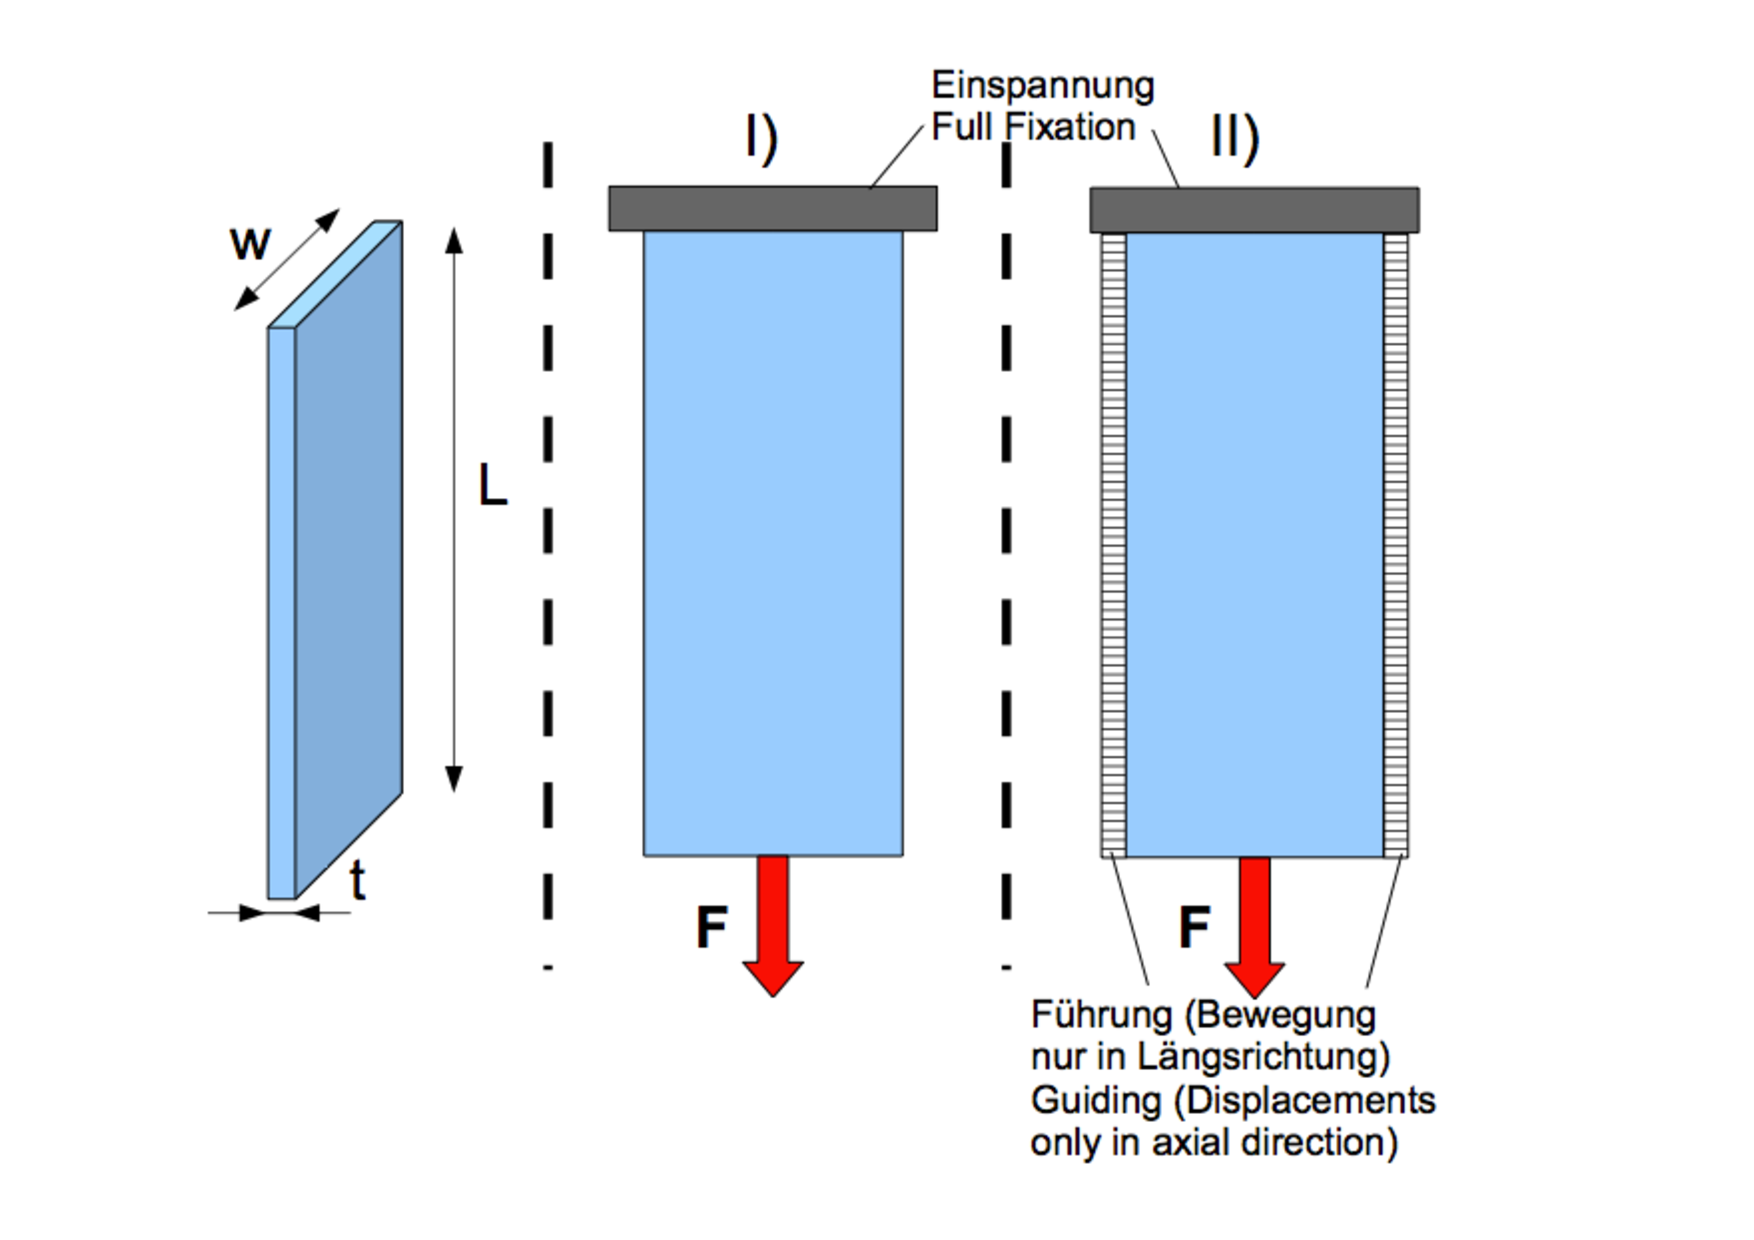
\includegraphics[scale=0.3]{images/structural_mechanics.pdf}
		\caption{Structural Mechanics}
		\label{fig:structuralmechanics}
	\end{center}
\end{figure}

Koordinatensystem: $x_1$: gegen mich, $x_2$: nach rechts, $x_3$ nach unten\\
Länge: $L = 10 cm$, Breite $w=2cm$, Dicke $t=2mm$\\

\textbf{Bestimme die Form des Spannungs- und Verzerrungstensor}\\

\textbf{Fall 1}\\
\begin{align}
	\epsilon_I^{eng} = (-e1, -e_1, e_3, 0, 0, 0)^T
\end{align}
Objekt wird nach unten in die Länge gezogen $e_3$. Dadurch zieht sich
das Objekt in $x_1$ und $x_2$ Richtung zusammen (identisch). Die hinteren
Nullen sind für die Eigenschaften der Scherrung reserviert.\\
\begin{align}
	\sigma_I = (0,0,s_3,0,0,0)^T
\end{align}
Es wirkt nur eine Kraft (Spannung) nach unten.\\

\textbf{Fall 2}\\
\begin{align}
	\epsilon_I^{eng} = (-e1, 0, e_3, 0, 0, 0)^T
\end{align}
Durch die Einspannung kann sich das Objekt in $x_2$ Richtung nicht
zusammenziehen.
\begin{align}
	\sigma_I = (0,s_2,s_3,0,0,0)^T
\end{align}
Daraus folgt, dass die Einspannung als Kraft in $x_2$ Richtung wirken muss.\\

\textbf{Berechnung Verzerrungs- und den Spannungstensor}\\
E-Modul: $E = 70 GPa$, Poissonzahl $\nu = 0.3$\\
Ausgehend von $\sigma = C \cdot \epsilon$:\\
Anhand Formel \ref{eq:elasticity}:
\begin{align}
	\mathbf{C} = \frac{E}{1 + \nu} \cdot \begin{pmatrix}
		\frac{1-\nu}{1-2\nu} & \frac{\nu}{1-2\nu} & \frac{\nu}{1-2\nu}\\
		\frac{\nu}{1-2\nu} & \frac{1-\nu}{1-2\nu} & \frac{\nu}{1-2\nu}\\
		\frac{\nu}{1-2\nu} & \frac{\nu}{1-2\nu} & \frac{1-\nu}{1-2\nu}
	\end{pmatrix}
\end{align}
Ergibt sich:
\begin{align}
	\frac{E}{1 + \nu} \cdot \begin{pmatrix}
		\frac{1-\nu}{1-2\nu} & \frac{\nu}{1-2\nu} & \frac{\nu}{1-2\nu}\\
		\frac{\nu}{1-2\nu} & \frac{1-\nu}{1-2\nu} & \frac{\nu}{1-2\nu}\\
		\frac{\nu}{1-2\nu} & \frac{\nu}{1-2\nu} & \frac{1-\nu}{1-2\nu}
	\end{pmatrix}
	\begin{pmatrix}
		-e_1\\ -e_1\\ e_3
	\end{pmatrix}
	=
	\begin{pmatrix}
		0\\ 0\\ s_3
	\end{pmatrix}
\end{align}
Linie 1 und 2 ergeben identische Formel, wobei Faktoren mit $C_{ij}$
geschrieben werden:
\begin{align}
	(C_{11} + C_{12}) \cdot (-e_1) + C_{12} \cdot e_3 = 0
\end{align}
2te Gleichung, Beachte $\frac{E}{1+\nu}$ ist wohl in den $C_{ij}$ versteckt:
\begin{align}
	2 \cdot C_{11} \cdot (-e_1) + C_{C_12} e_3 = s_3
\end{align}
Bei der Auflösung des Gleichungssystem wird dass Prinzip der Mut zur Lücke laut
der Formel 379 nach Dr. D. Strebel angewahnt!